% Исследовательская часть
\section{Описание исследования}

\hspace{1.25cm}
Было выполнено исследование зависимости производительности разработанного ПО (в терминах количества обработанных страниц в единицу времени) от количества дополнительных потоков. Количество дополнительных потоков изменялось от 0 (вычисление в основном потоке), до $4\cdot 16 = 64$, где $16$ --- количество логических ядер используемой ЭВМ (см листинг~\ref{lst:research} и график~\ref{fig:img_graph}).

\vspace{0.25cm}
\begin{lstlisting}[caption=Результаты замеров времени на разном количестве потоков, label=lst:research]
Taking measurements (number of logical cores = 16, number of links = 100):
Running on the main thread Execution time: 06/290003 sec
Number of threads: 1 Execution time: 30.503609 sec
Number of threads: 2 Execution time: 13.407696 sec
Number of threads: 4 Execution time: 7.321394 sec
Number of threads: 8 Execution time: 4.626752 sec
Number of threads: 16 Execution time: 3.882306 sec
Number of threads: 32 Execution time: 4.112705 sec
Number of threads: 64 Execution time: 3.792753 sec
\end{lstlisting}

\vspace{-0.25cm}
\begin{figure}[h]
    \centering
    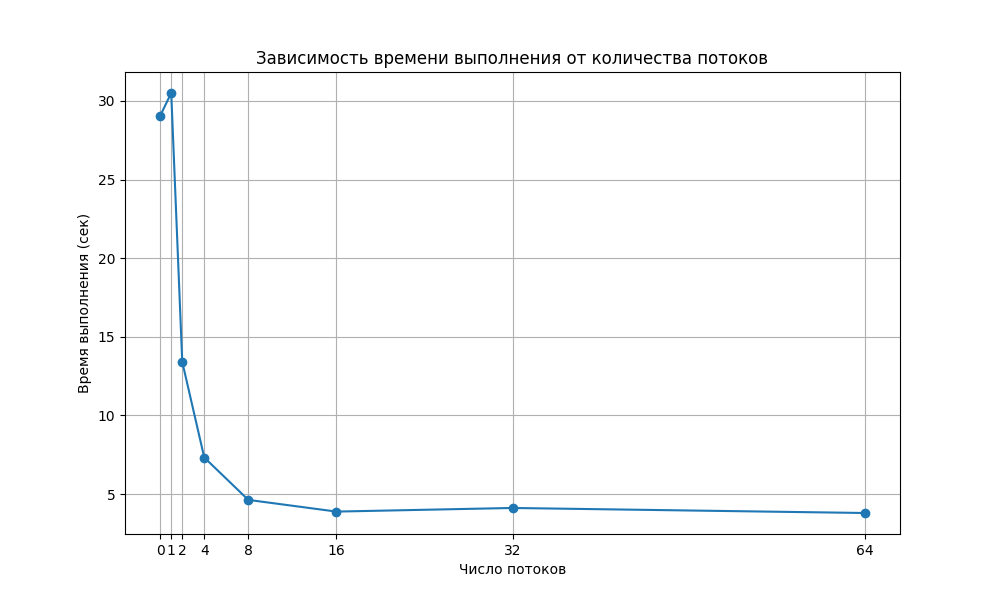
\includegraphics[width=\linewidth]{img/graph.png}
    \caption{График замеров времени на разном количестве потоков}
    \label{fig:img_graph}
\end{figure}

\subsection*{Анализ производительности}

\hspace{1.25cm}
На основе представленных данных о времени выполнения загрузки 100 страниц при разном количестве потоков сформулируем несколько выводов:

\subsubsection*{Последовательная загрузка}

\begin{enumerate}
    \item Запуск на основном потоке занял 29.06 секунд.
    \item При использовании 1 потока время увеличилось до 30.50 секунд. Это может указывать на дополнительные накладные расходы на создание потоков и их управление, которые перекрывают выгоду от работы при одном потоке.
\end{enumerate}

\subsubsection*{Увеличение числа потоков}

\hspace{1.25cm}
Время выполнения значительно сокращается при увеличении числа потоков до 16. Например:

\begin{enumerate}
    \item 2 потока – 13.41 секунд (почти вдвое быстрее, чем один поток).
    \item 4 потока – 7.32 секунд.
    \item 8 потоков – 4.63 секунд.
    \item 16 потоков – 3.88 секунд.
\end{enumerate}

Это демонстрирует эффективное масштабирование производительности, особенно при увеличении числа потоков до числа логических ядер процессора (16).

\subsubsection*{Сверх числа логических ядер}

\hspace{1.25cm}
При увеличении числа потоков до 32 и 64 наблюдается незначительное ухудшение производительности:

\begin{enumerate}
    \item 32 потока – 4.11 секунд.
    \item 64 потока – 3.79 секунд.
\end{enumerate}

Это явление можно объяснить накладными расходами на планирование потоков и синхронизацию между ними. Увеличение числа потоков сверх числа логических ядер (16) не даёт значительного прироста и даже начинает снижать эффективность~\cite{silberschatz}.

\subsubsection*{Выводы}

\begin{enumerate}
    \item Оптимальное число потоков для данного теста – около 16, что соответствует числу логических ядер процессора. Увеличение числа потоков свыше этого значения не приводит к улучшению производительности.
    \item В случае с малым числом потоков (1 и 2), многопоточность даёт значительный прирост по сравнению с последовательным запуском, однако использование одного потока может даже замедлять выполнение из-за накладных расходов на многопоточность.
    \item Важно учитывать баланс между количеством потоков и ресурсами системы, чтобы избежать чрезмерной нагрузки на планировщик и неэффективного использования ядер.
\end{enumerate}